\problemname{Snóker}
\illustration{0.3}{framestart}{Mynd fengin af \href{https://www.flickr.com/photos/192927703@N08/51223529455}{flickr.com}}

Arnar hefur verið að horfa á snóker nýlega.
Í snóker er spilað á stóru rétthyrningslaga leikborði og notast spilarar við kjuða, sem er í raun bara sérsmíðað prik.
Leikborðið er $140{,}5$ tommur að lengd og $70$ tommur að breidd.
Það eru sex vasar á leikborðinu, einn í hverju horni og svo tveir fyrir miðju á hvorri langhlið fyrir sig.

Á borðinu eru einnig kúlur í mörgum litum og hefur hver litur ákveðna merkingu.
Radíus kúlnanna er $1$ tomma.
Litirnir eru rauður, gulur, grænn, brúnn, blár, bleikur og svartur.
Einnig er hvít kúla á borðinu og er hún eina kúlan sem má slá í með kjuðanum.
Leikmenn pota þá öðrum enda kjuðans í hvítu kúluna þannig að hún rúlli áfram eftir borðinu.
Hún getur rekist á og skoppað af köntum borðsins, en einnig getur hún rekist á og haft áhrif á hinar kúlurnar.
Markmið leiksins er að hitta hvítu kúlunni í lituðu kúlurnar þannig þær fari ofan í vasa borðsins.
Kúlurnar gefa mismunandi fjölda stiga, mismunandi eftir lit kúlunnar, þegar þær komast ofan í vasa, eins og má sjá í eftirfarandi töflu.

\begin{center}
\begin{tabular}{|l|l|}
\hline
    Litur   & Stig \\ \hline
    Rauður  & $1$  \\ \hline
    Gulur   & $2$  \\ \hline
    Grænn   & $3$  \\ \hline
    Brúnn   & $4$  \\ \hline
    Blár    & $5$  \\ \hline
    Bleikur & $6$  \\ \hline
    Svartur & $7$  \\ \hline
\end{tabular}
\end{center}

Í hvert sinn sem hvítu kúlunni er skotið er ákveðinn litur sem skal hitta fyrst með hvítu kúlunni.
Alltaf þegar leikmaður hittir réttum lit ofan í vasa fær hann að skjóta aftur, annars tekur hinn leikmaðurinn við.
Ef það er rauð kúla á borðinu þegar leikmaður byrjar umferð sína, þarf leikmaður fyrst að hitta í rauðu kúlu
og ef leikmanni tekst að koma rauðri kúlu í vasa fær leikmaður að velja lit, ekki rauðan, fyrir næsta skot.
Ef leikmaður nær litaðri kúlu ofan í vasa eftir rauðri, er litaða kúlan sett aftur á borðið eftir að stig eru gefin.
Eftir skotið á þá aftur að hitta rauða kúlu fyrst.
Þegar allar rauðar kúlur eru farnar af borðinu skal skjóta hinum kúlunum niður í sömu röð og má sjá í töflunni að ofan.

Ef hvíta kúlan rekst fyrst í réttan lit þá flokkast skotið sem \texttt{HIT}.
Ef hvíta kúlan rekst fyrst í rangan lit þá flokkast skotið sem \texttt{FOUL}.
Ef hvíta kúlan rekst ekki í neina kúlu þá flokkast skotið sem \texttt{MISS}.
Athugaðu að hvíta kúlan má rekast í kanta eins oft og mögulegt er, bæði fyrir og eftir að hún rekst í fyrstu kúluna.

Eitt af markmiðum leiksins er að \emph{snókera} andstæðinginn með því að skjóta hvítu kúlunni þannig sé illa staðsett fyrir andstæðinginn.
Þá getur reynst erfitt að hitta réttu kúluna og ekki víst að beint skot sé í boði.
Þá er venjulega skotið hvítu kúlunni þannig hún skoppi af köntum borðsins einu sinni eða oftar áður en hún lendir á kúlu.
Þar sem það getur reynst erfitt að sjá skoppin fyrir sér vill Arnar að þú segir sér hvort hvíta kúlan hitti rétta kúlu.

Þú færð gefna núverandi stöðu borðsins, hvaða lit leikmaður á að hitta fyrst og lýsingu á ferð hvítu kúlunnar eftir að kjuðanum er slegið í hana.
Segðu til hvort skotið sé \texttt{HIT}, \texttt{FOUL} eða \texttt{MISS}.
Til að einfalda verkefnið skal gera ráð fyrir að það séu engir vasar á borðinu, þannig hvíta kúlan fer aldrei ofan í vasa, heldur skoppar hún alltaf af kanti þegar hún kemur að honum.

\section*{Inntak}
Fyrsta línan inniheldur eina heiltölu $n$, þar sem $2 \leq n \leq 22$, sem táknar fjölda kúlna á borðinu.
Næst fylgja $n$ línur.
Hver lína inniheldur lit kúlunnar og tvær rauntölur $x_i$, þar sem $1 \leq x_i \leq 69$, og $y_i$, þar sem $1 \leq y_i \leq 139{,}5$, sem eru aðskilnar með bili og tákna staðsetningu $i$-tu kúlunnar á borðinu.
Svo kemur lína með litnum sem á að hitta fyrst.
Að lokum kemur lína með tveimur rauntölum $v_x$ og $v_y$, þar sem $-1\,000 \leq v_x, v_y \leq 1\,000$, sem eru aðskilnar með bili og tákna hversu langt hvíta kúlann ferðast á hvorum ás fyrir sig.

Litum kúlnanna er lýst í inntaki með strengjunum \texttt{white}, \texttt{red}, \texttt{yellow}, \texttt{green}, \texttt{brown}, \texttt{blue}, \texttt{pink} og \texttt{black}.
Það geta verið allt að $15$ rauðar kúlur á borðinu, en í mesta lagi $1$ af hverjum öðrum lit.
Hvíta kúlan er alltaf á borðinu og einnig er allavega ein kúla á borðinu með litinn sem á að hitta fyrst.
Staðsetning hverrar kúlu er gefin sem fjarlægðin frá efra vinstra horna borðsins að miðju kúlunnar, í tommum.
Efra vinstra hornið er því á staðsetningunni $(0; 0)$ og neðra hægra hornið á staðsetningunni $(70; 140{,}5)$.
Gera má ráð fyrir að kúlurnar skarist ekki en þær mega snertast.
Hvíta kúlan mun hinsvegar ekki snerta neina kúlu í upphafi.
Allar rauntölur eru gefnar með nákvæmlega þremur aukastöfum.

\section*{Úttak}
Skrifaðu út \texttt{HIT} ef hvíta kúlan klessir fyrst á réttum lit,
\texttt{FOUL} ef hvíta kúlan klessir í röngum lit fyrst eða
\texttt{MISS} ef hvíta kúlan klessir ekki á neina kúlu.
Gera má ráð fyrir að svarið breytist ekki ef staðsetning kúlna breytist um minna en $10^{-3}$ tommur og er svarið því aldrei tvírætt.

\section*{Stigagjöf}
\begin{tabular}{|l|l|l|}
\hline
Hópur & Stig & Takmarkanir \\ \hline
1     & 30   & Hvíta kúlan fer ekki nógu langt til að klessa á kant. Annaðhvort $v_x = 0$ eða $v_y = 0$. \\ \hline
2     & 20   & Annaðhvort $v_x = 0$ eða $v_y = 0$. \\ \hline
3     & 25   & Hvíta kúlan fer ekki nógu langt til að klessa á kant. \\ \hline
4     & 25   & Engar frekari takmarkanir\\ \hline
\end{tabular}

\section*{Útskýringar á sýnidæmum}
Fyrsta sýnidæmið fellur undir hóp $1$. Svarið er \texttt{HIT} því hvíta kúlan hittir svörtu kúluna fyrst.
\begin{figure}[ht!]
  \centering
    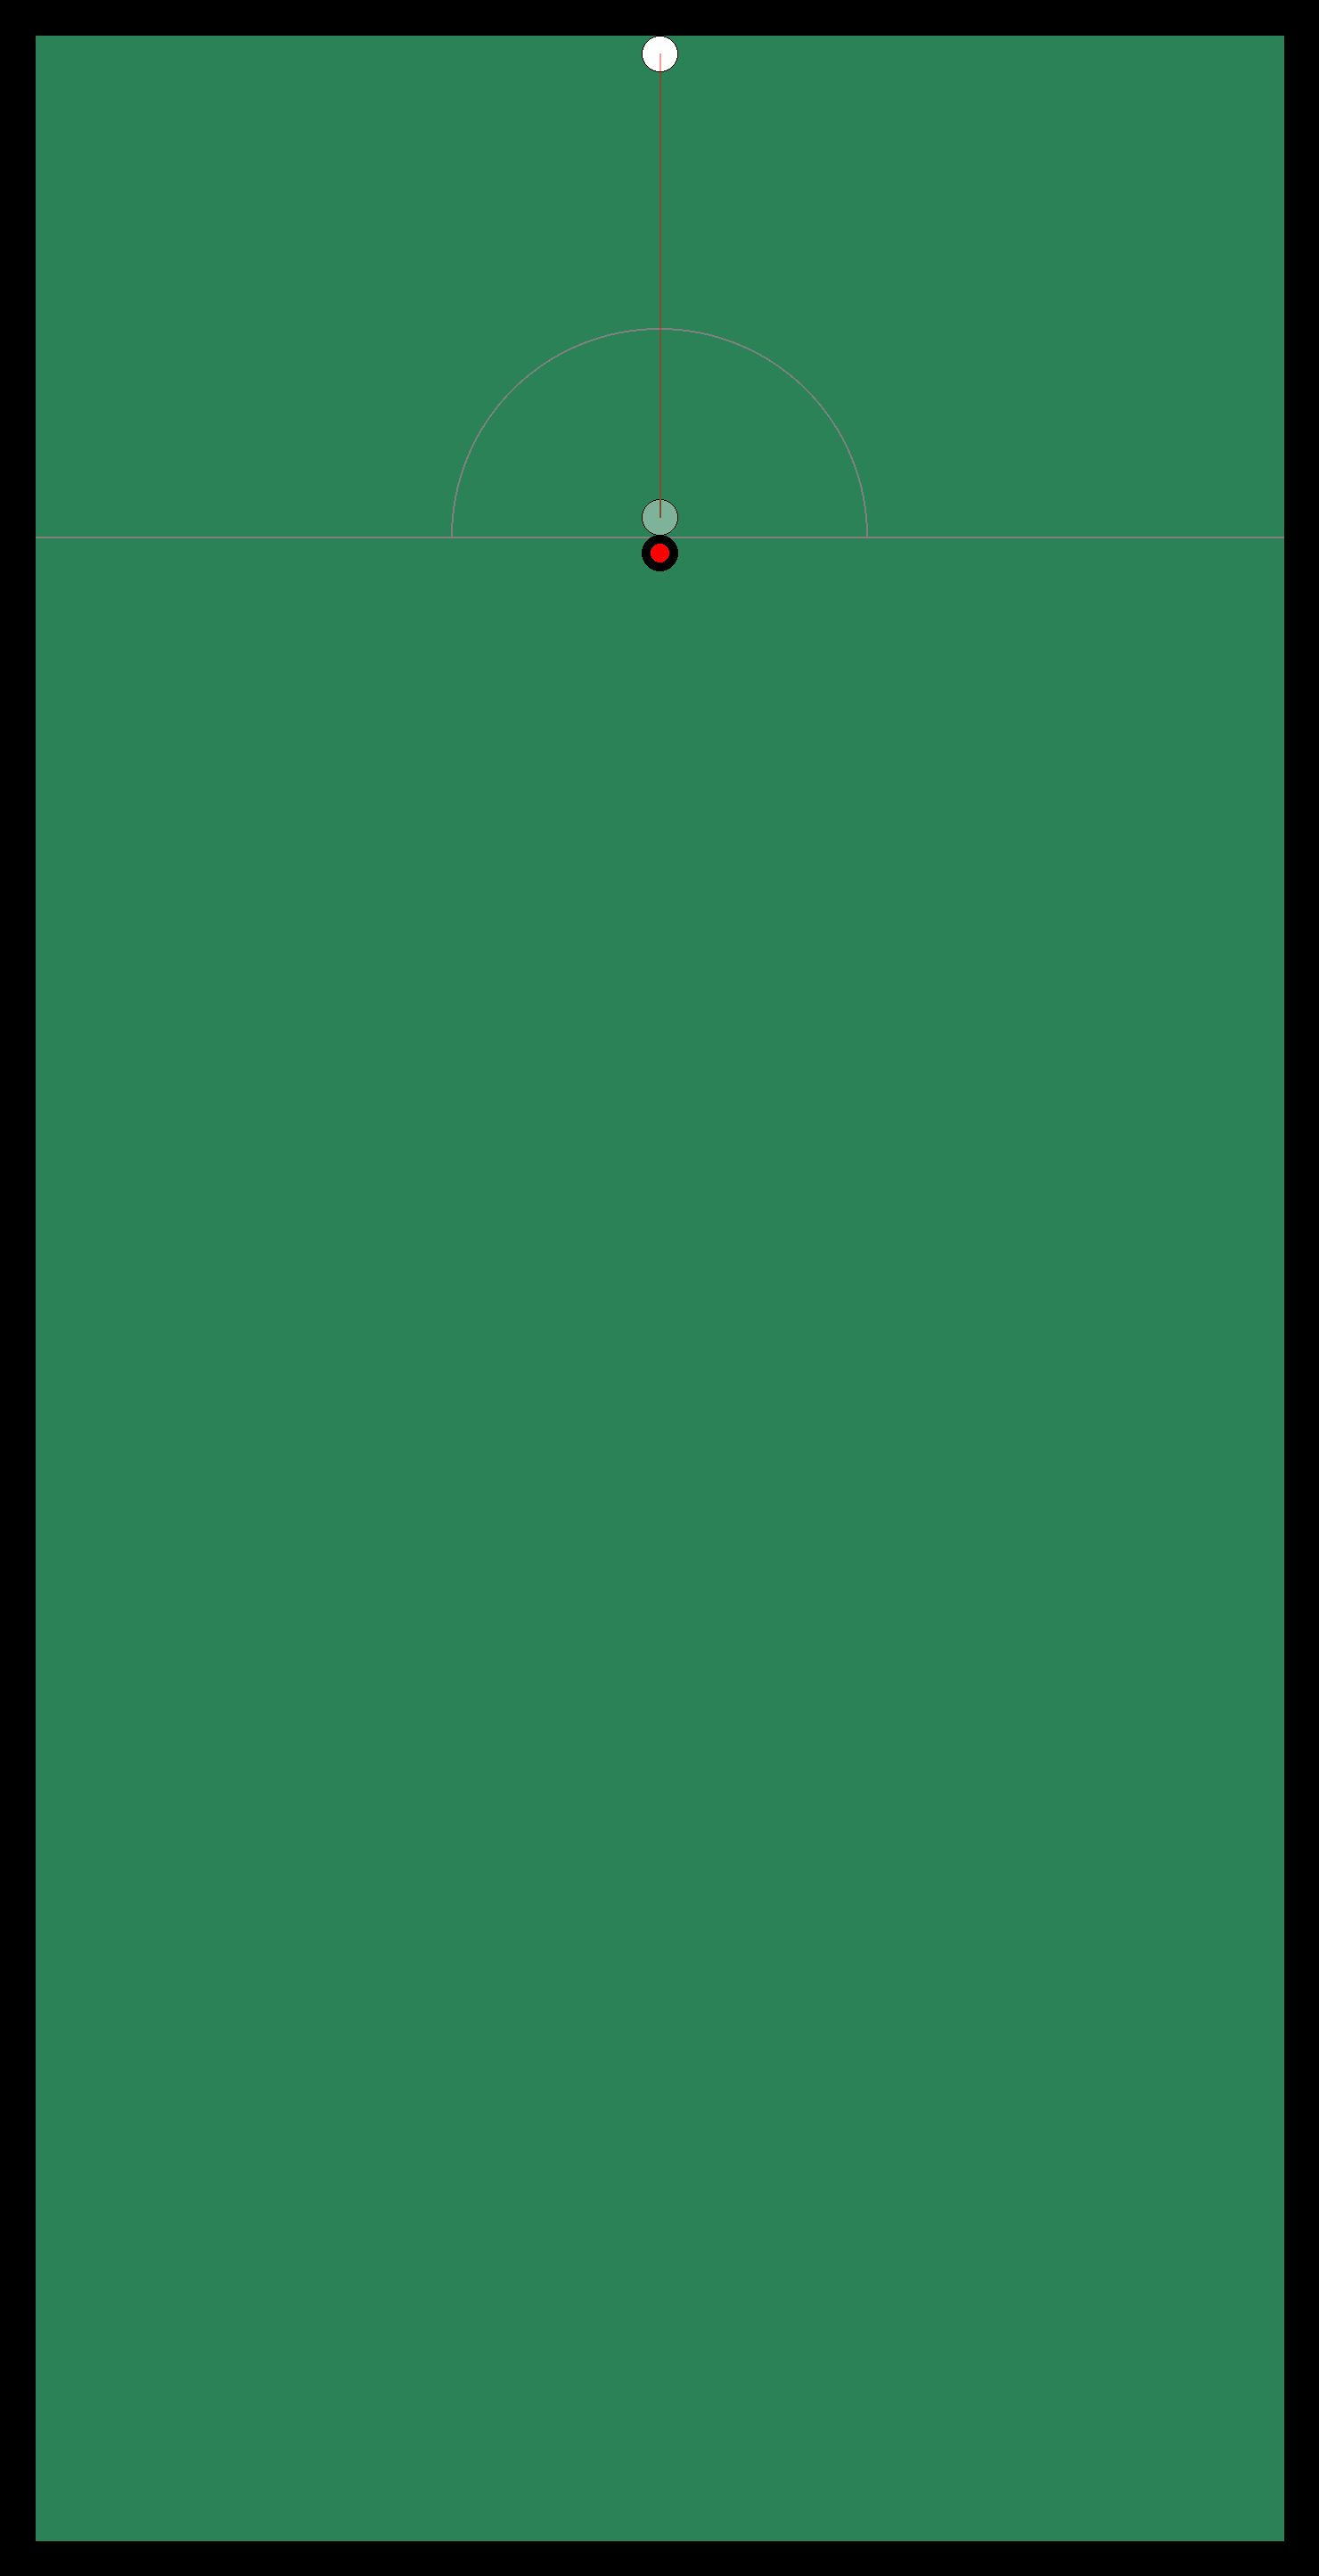
\includegraphics[width=0.7\textwidth]{sample1}
  \caption{Sýnidæmi 1}
\end{figure}

Annað sýnidæmið fellur undir hóp $2$. Hvíta kúlan skoppar fyrst af neðri kanti og heldur svo áfram upp. Svarið er \texttt{FOUL} því hvíta kúlan hittir bleiku kúluna fyrst.
\begin{figure}[ht!]
  \centering
    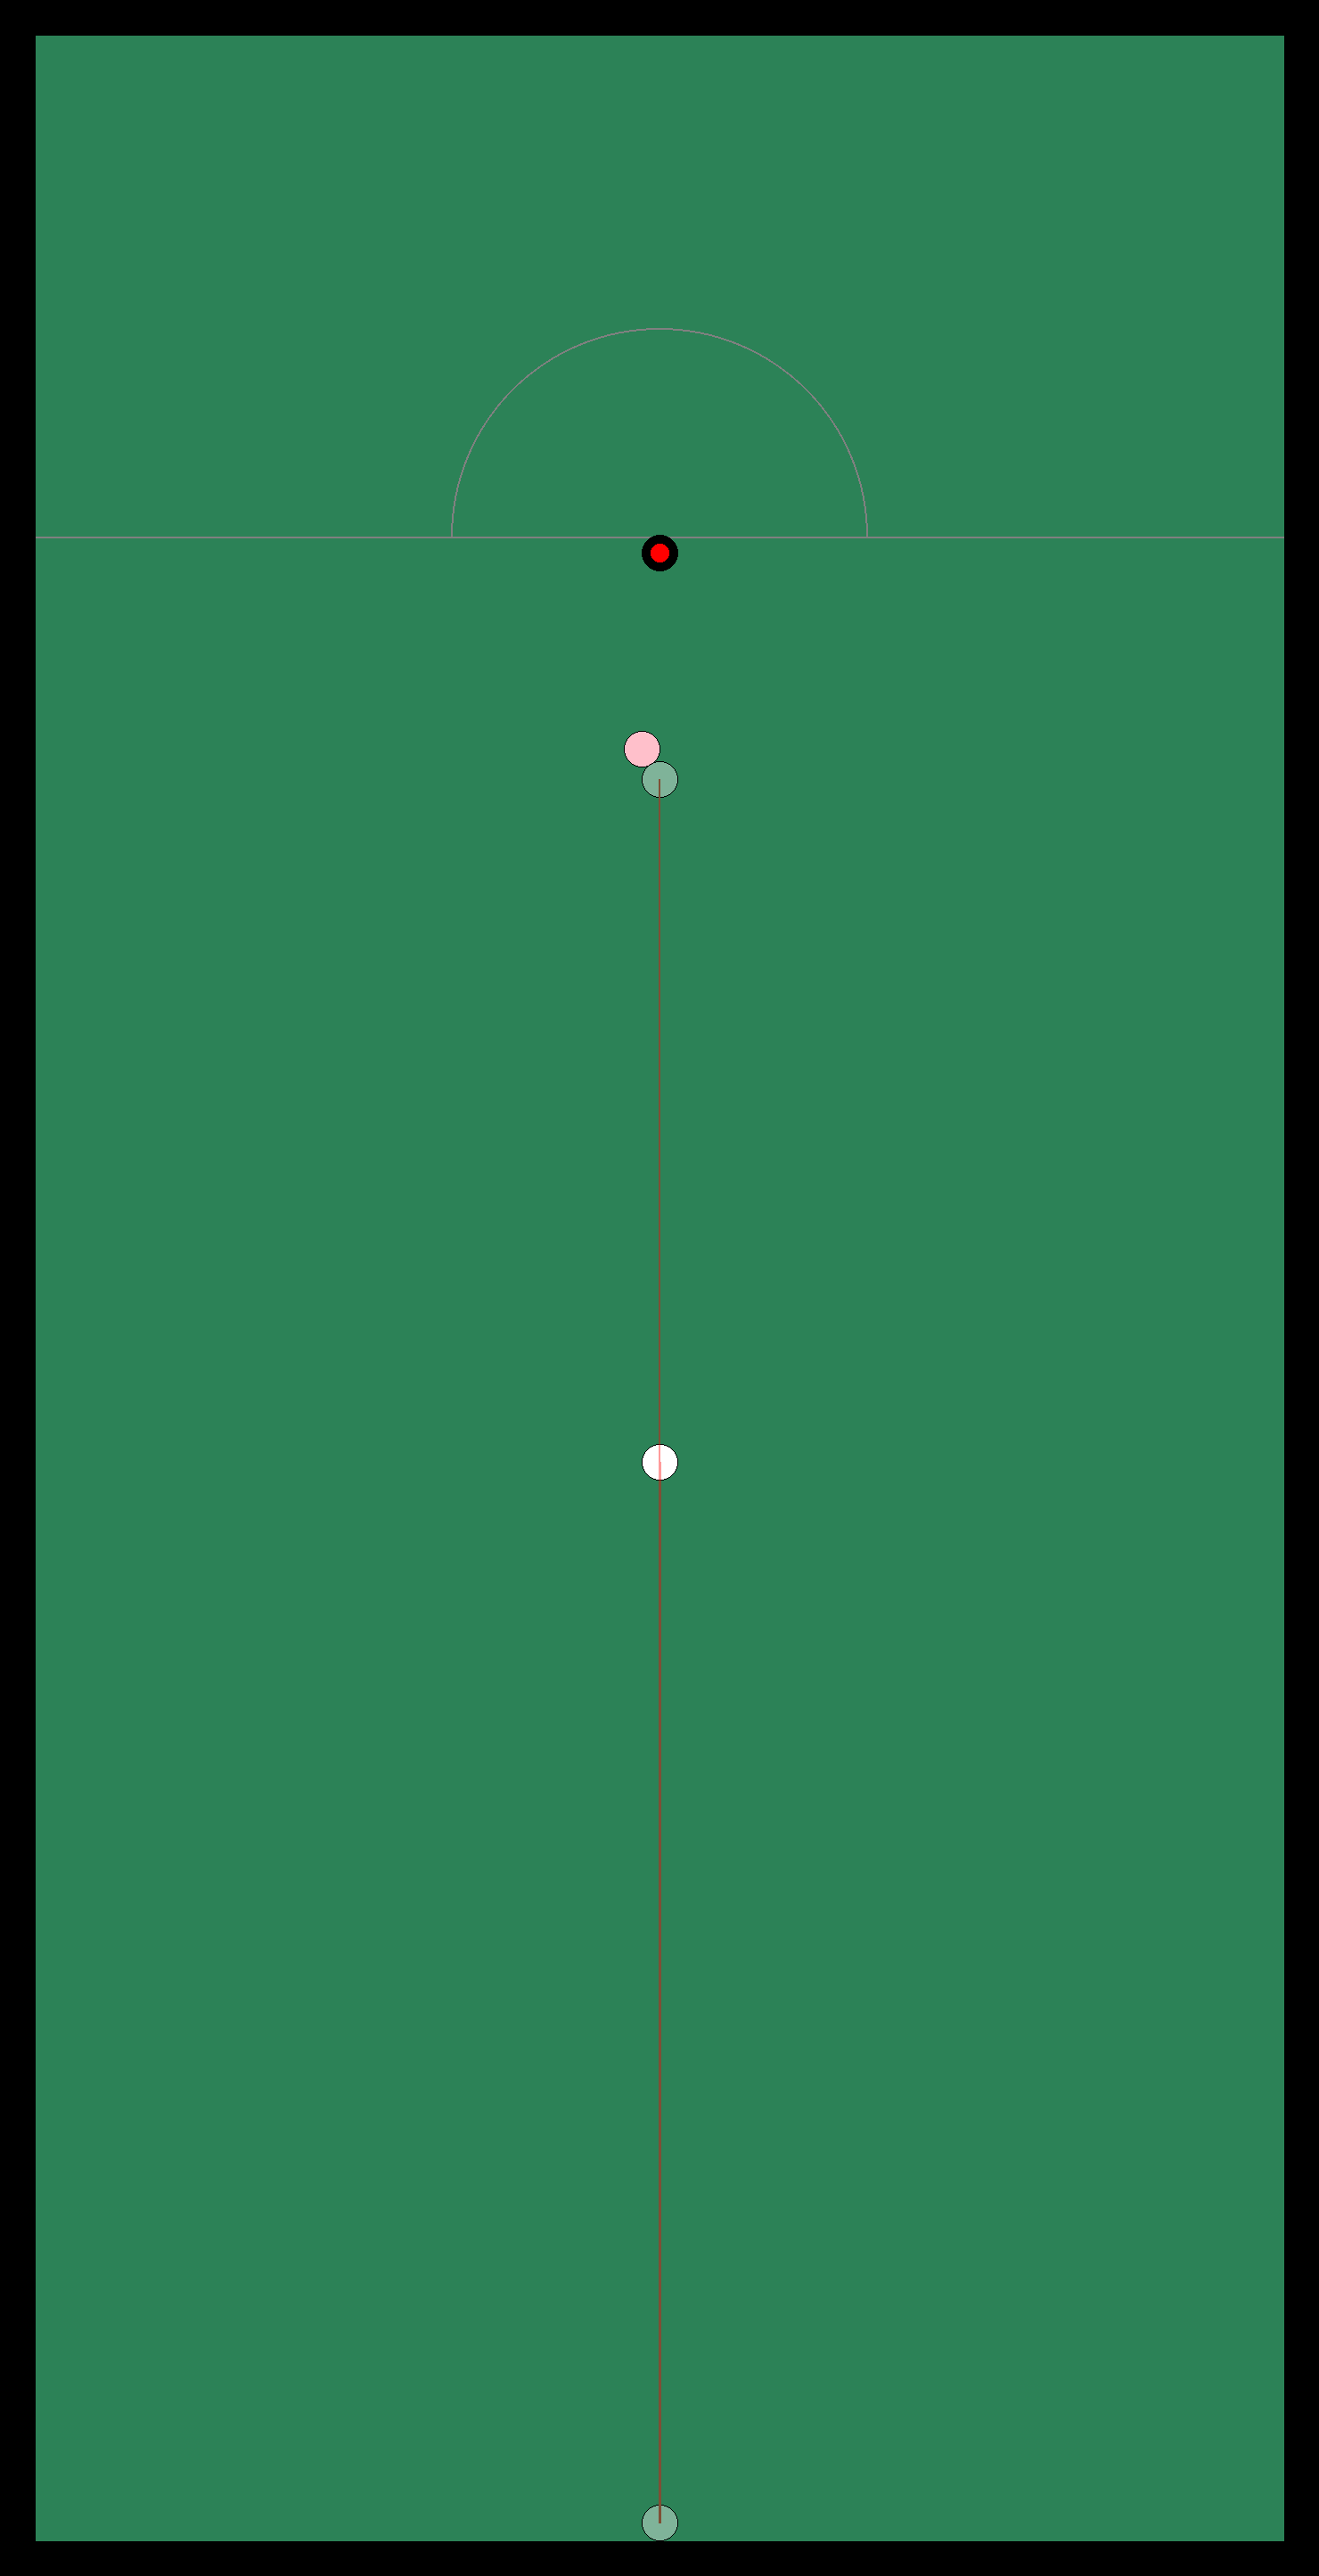
\includegraphics[width=0.7\textwidth]{sample2}
  \caption{Sýnidæmi 2}
\end{figure}

Þriðja sýnidæmið fellur undir hóp $3$. Hvíta kúlan fer á milli grænu kúlunnar og brúnu kúlunnar. Svarið er \texttt{FOUL} því hvíta kúlan hittir bláu kúluna fyrst.
\begin{figure}[ht!]
  \centering
    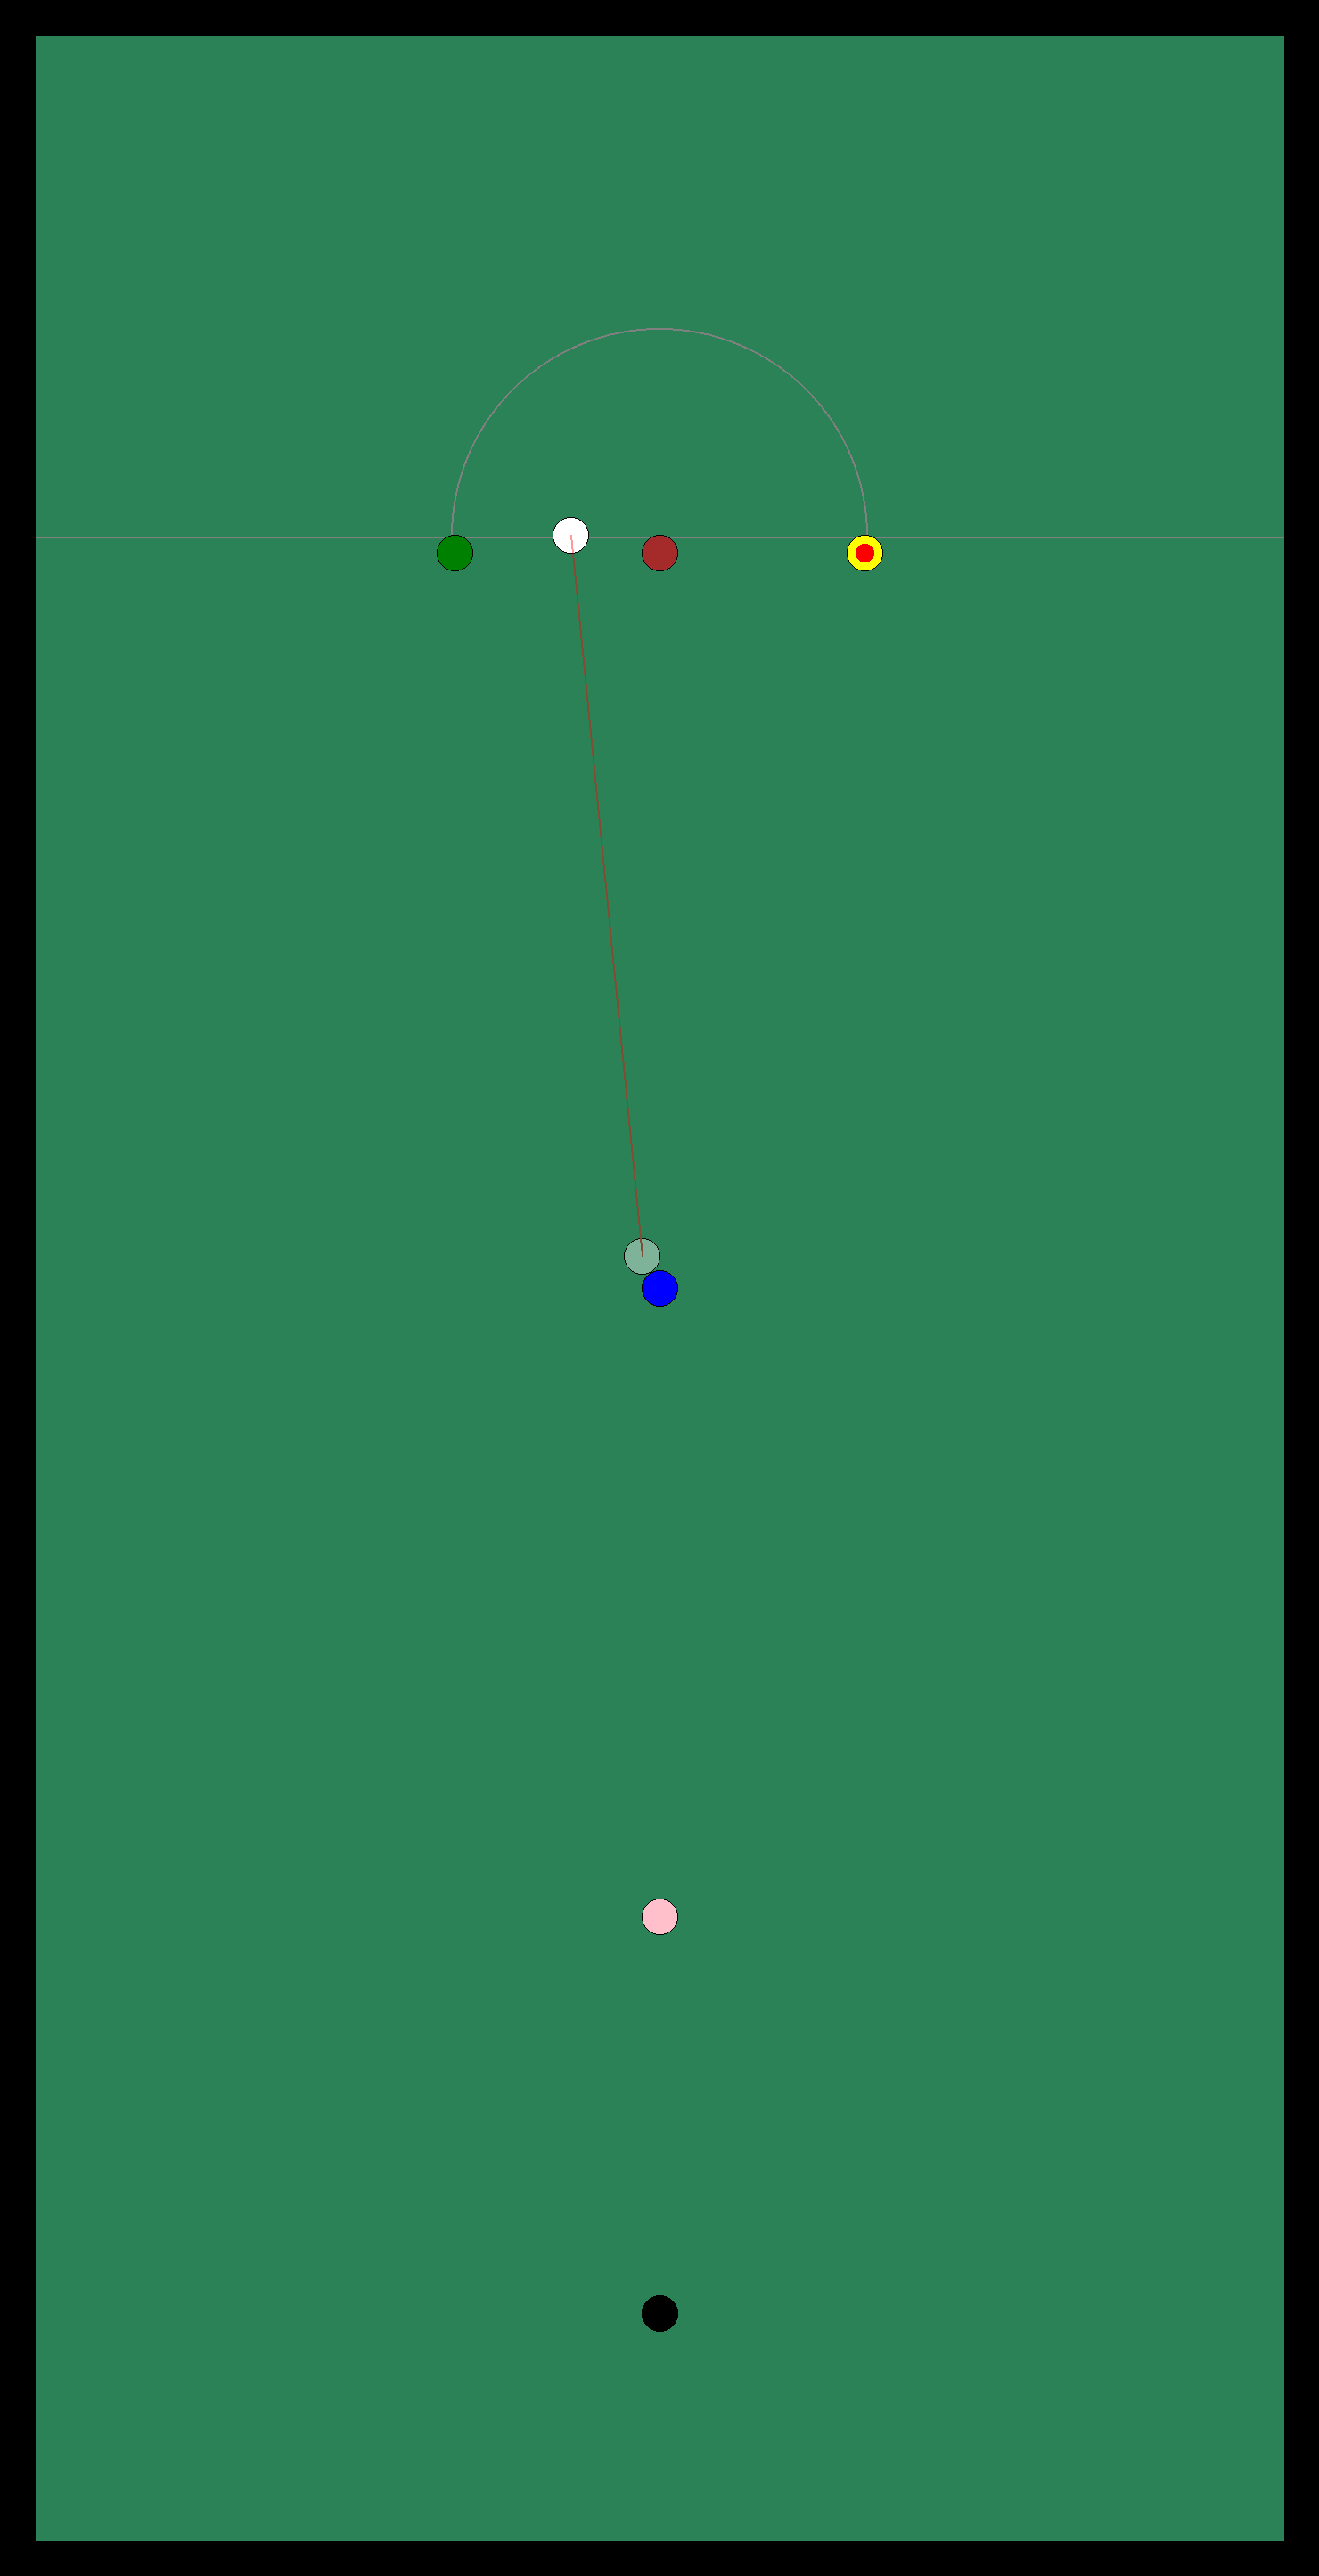
\includegraphics[width=0.7\textwidth]{sample3}
  \caption{Sýnidæmi 3}
\end{figure}

Fjórða sýnidæmið fellur undir hóp $4$. Hvíta kúlan fer fyrst milli brúnu kúlunnar og gulu kúlunnar, og skoppar fyrst af neðri kanti, svo vinstri kanti.
Næst fer hvíta kúlan framhjá grænu kúlunni, skoppar af efri kanti og fer  milli grænu kúlunnar og brúnu kúlunnar.
Að lokum skoppar hvíta kúlan af neðri kantinum og ferðast nánast upp að hægri kanti þar sem hún stöðvar.
Svarið er \texttt{MISS} því hvíta kúlan hittir enga kúlu áður en hún stöðvar.
\begin{figure}[ht!]
  \centering
    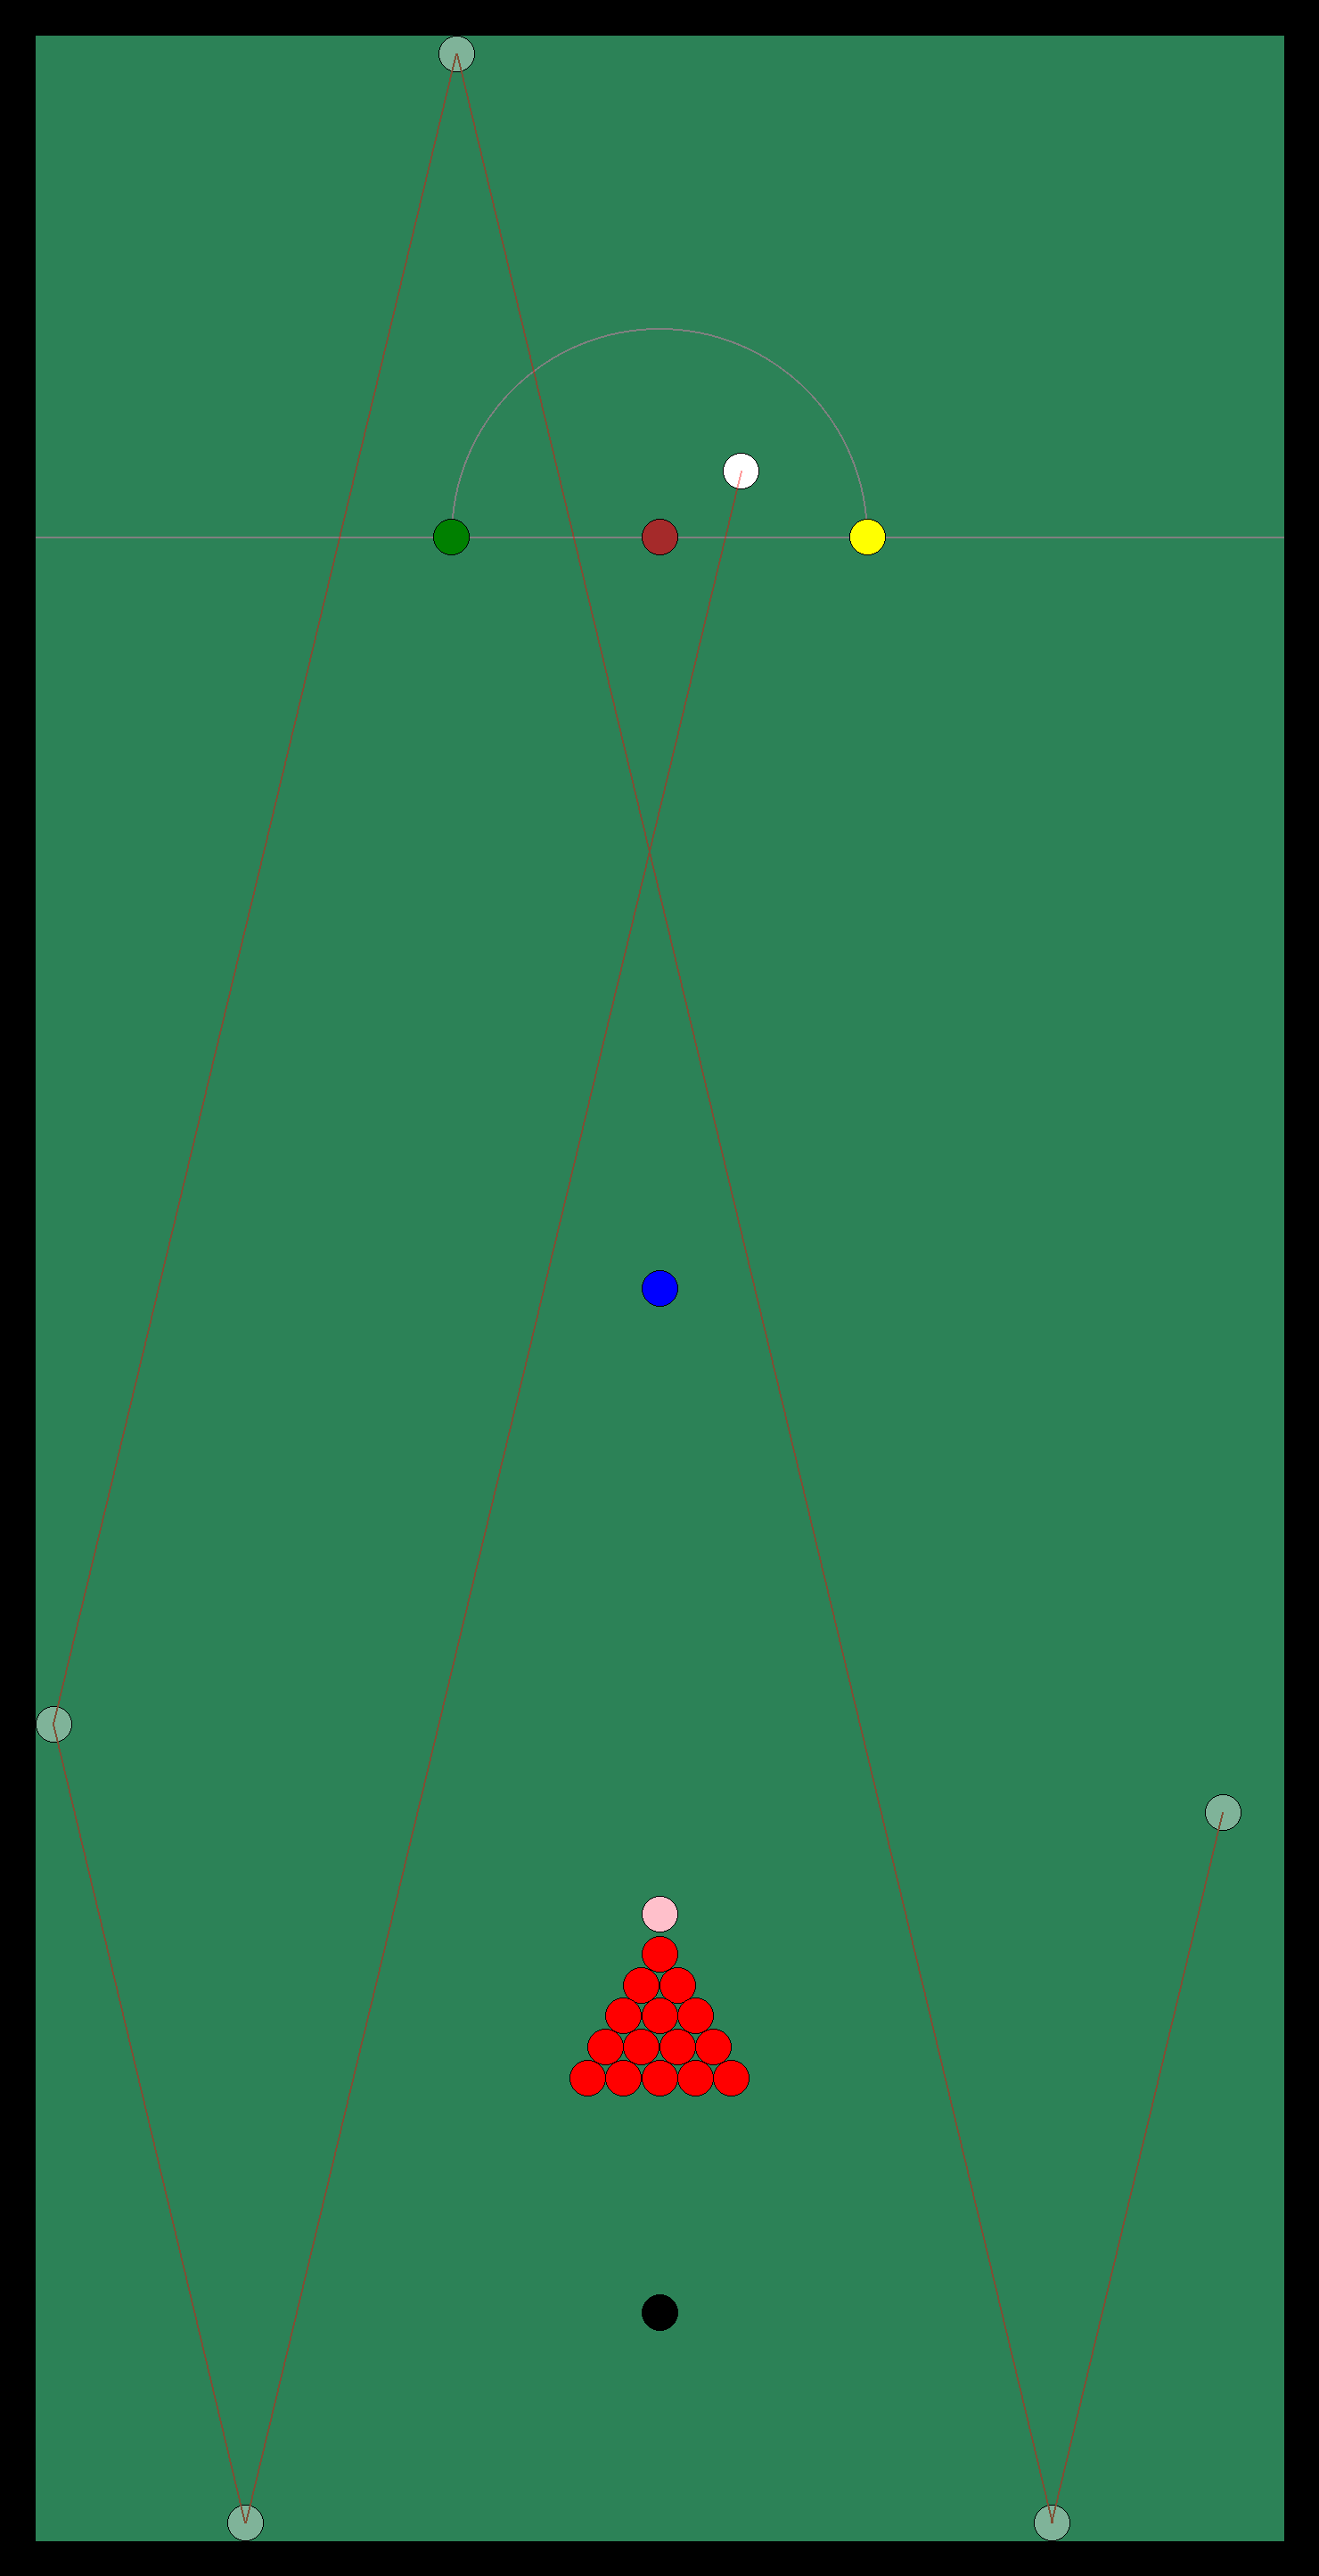
\includegraphics[width=0.7\textwidth]{sample4}
  \caption{Sýnidæmi 4}
\end{figure}
